\documentclass[tikz,border=3pt]{standalone}
    \usepackage[tt=false,type1=true]{libertine}
    \usepackage[libertine]{newtxmath}
    \usepackage{pgfplots}
    \usepgfplotslibrary{groupplots}
    \pgfplotsset{compat=1.18}
    \definecolor{accent}{HTML}{466E8B}
    \definecolor{graybar}{HTML}{A1A1A1}
    \begin{document}
    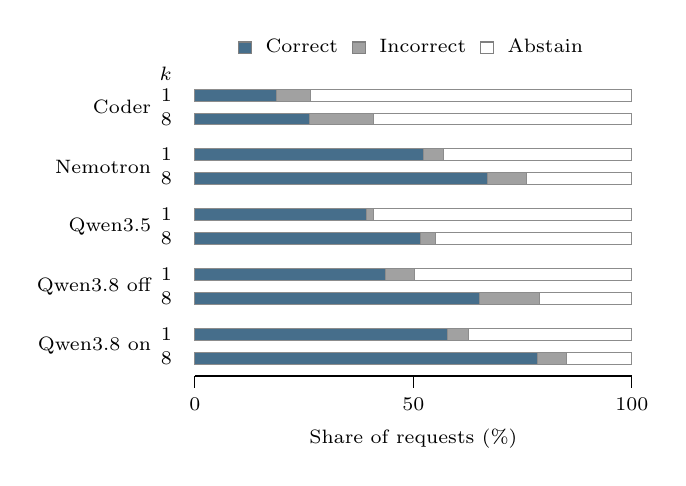
\begin{tikzpicture}
    \begin{axis}[
     width=5.55cm,height=3.8cm,scale only axis,
     xmin=0,xmax=100,ymin=.5,ymax=5.5,
     xtick={0,50,100},ytick={5,4,3,2,1},
     yticklabels={Coder,Nemotron,Qwen3.5,Qwen3.8 off,Qwen3.8 on},
     tick label style={font=\fontsize{7.5}{8.5}\selectfont},
     yticklabel style={xshift=-8pt},
     label style={font=\fontsize{7.5}{8.5}\selectfont},
     xlabel={Share of requests (\%)},
     axis x line*=bottom,axis y line*=left,
     y axis line style={draw=none},ytick style={draw=none},
     tick align=outside,xtick style={black,line width=.45pt},
     axis line style={black,line width=.5pt},clip=false,
     legend columns=3,
     legend style={at={(.5,1.03)},anchor=south,font=\fontsize{7.2}{8.2}\selectfont,draw=none,column sep=3pt},
     legend image code/.code={\draw[#1] (0cm,-.07cm) rectangle (.16cm,.07cm);}
    ]
    \addlegendimage{draw=black!50,fill=accent}\addlegendentry{Correct}
    \addlegendimage{draw=black!50,fill=graybar}\addlegendentry{Incorrect}
    \addlegendimage{draw=black!50,fill=white}\addlegendentry{Abstain}
    \path[fill=accent,draw=black!45,line width=.25pt] (axis cs:0.000000000,5.100000000) rectangle (axis cs:18.553459119,5.300000000);
\path[fill=graybar,draw=black!45,line width=.25pt] (axis cs:18.553459119,5.100000000) rectangle (axis cs:26.415094340,5.300000000);
\path[fill=white,draw=black!45,line width=.25pt] (axis cs:26.415094340,5.100000000) rectangle (axis cs:100.000000000,5.300000000);
\node[anchor=east,font=\fontsize{7}{8}\selectfont] at (axis cs:-3,5.200000000) {1};
\path[fill=accent,draw=black!45,line width=.25pt] (axis cs:0.000000000,4.700000000) rectangle (axis cs:26.100628931,4.900000000);
\path[fill=graybar,draw=black!45,line width=.25pt] (axis cs:26.100628931,4.700000000) rectangle (axis cs:40.880503145,4.900000000);
\path[fill=white,draw=black!45,line width=.25pt] (axis cs:40.880503145,4.700000000) rectangle (axis cs:100.000000000,4.900000000);
\node[anchor=east,font=\fontsize{7}{8}\selectfont] at (axis cs:-3,4.800000000) {8};
\path[fill=accent,draw=black!45,line width=.25pt] (axis cs:0.000000000,4.100000000) rectangle (axis cs:52.201257862,4.300000000);
\path[fill=graybar,draw=black!45,line width=.25pt] (axis cs:52.201257862,4.100000000) rectangle (axis cs:56.918238994,4.300000000);
\path[fill=white,draw=black!45,line width=.25pt] (axis cs:56.918238994,4.100000000) rectangle (axis cs:100.000000000,4.300000000);
\node[anchor=east,font=\fontsize{7}{8}\selectfont] at (axis cs:-3,4.200000000) {1};
\path[fill=accent,draw=black!45,line width=.25pt] (axis cs:0.000000000,3.700000000) rectangle (axis cs:66.981132075,3.900000000);
\path[fill=graybar,draw=black!45,line width=.25pt] (axis cs:66.981132075,3.700000000) rectangle (axis cs:75.786163522,3.900000000);
\path[fill=white,draw=black!45,line width=.25pt] (axis cs:75.786163522,3.700000000) rectangle (axis cs:100.000000000,3.900000000);
\node[anchor=east,font=\fontsize{7}{8}\selectfont] at (axis cs:-3,3.800000000) {8};
\path[fill=accent,draw=black!45,line width=.25pt] (axis cs:0.000000000,3.100000000) rectangle (axis cs:39.308176101,3.300000000);
\path[fill=graybar,draw=black!45,line width=.25pt] (axis cs:39.308176101,3.100000000) rectangle (axis cs:40.880503145,3.300000000);
\path[fill=white,draw=black!45,line width=.25pt] (axis cs:40.880503145,3.100000000) rectangle (axis cs:100.000000000,3.300000000);
\node[anchor=east,font=\fontsize{7}{8}\selectfont] at (axis cs:-3,3.200000000) {1};
\path[fill=accent,draw=black!45,line width=.25pt] (axis cs:0.000000000,2.700000000) rectangle (axis cs:51.572327044,2.900000000);
\path[fill=graybar,draw=black!45,line width=.25pt] (axis cs:51.572327044,2.700000000) rectangle (axis cs:55.031446541,2.900000000);
\path[fill=white,draw=black!45,line width=.25pt] (axis cs:55.031446541,2.700000000) rectangle (axis cs:100.000000000,2.900000000);
\node[anchor=east,font=\fontsize{7}{8}\selectfont] at (axis cs:-3,2.800000000) {8};
\path[fill=accent,draw=black!45,line width=.25pt] (axis cs:0.000000000,2.100000000) rectangle (axis cs:43.710691824,2.300000000);
\path[fill=graybar,draw=black!45,line width=.25pt] (axis cs:43.710691824,2.100000000) rectangle (axis cs:50.314465409,2.300000000);
\path[fill=white,draw=black!45,line width=.25pt] (axis cs:50.314465409,2.100000000) rectangle (axis cs:100.000000000,2.300000000);
\node[anchor=east,font=\fontsize{7}{8}\selectfont] at (axis cs:-3,2.200000000) {1};
\path[fill=accent,draw=black!45,line width=.25pt] (axis cs:0.000000000,1.700000000) rectangle (axis cs:65.094339623,1.900000000);
\path[fill=graybar,draw=black!45,line width=.25pt] (axis cs:65.094339623,1.700000000) rectangle (axis cs:78.930817610,1.900000000);
\path[fill=white,draw=black!45,line width=.25pt] (axis cs:78.930817610,1.700000000) rectangle (axis cs:100.000000000,1.900000000);
\node[anchor=east,font=\fontsize{7}{8}\selectfont] at (axis cs:-3,1.800000000) {8};
\path[fill=accent,draw=black!45,line width=.25pt] (axis cs:0.000000000,1.100000000) rectangle (axis cs:57.861635220,1.300000000);
\path[fill=graybar,draw=black!45,line width=.25pt] (axis cs:57.861635220,1.100000000) rectangle (axis cs:62.578616352,1.300000000);
\path[fill=white,draw=black!45,line width=.25pt] (axis cs:62.578616352,1.100000000) rectangle (axis cs:100.000000000,1.300000000);
\node[anchor=east,font=\fontsize{7}{8}\selectfont] at (axis cs:-3,1.200000000) {1};
\path[fill=accent,draw=black!45,line width=.25pt] (axis cs:0.000000000,0.700000000) rectangle (axis cs:78.301886792,0.900000000);
\path[fill=graybar,draw=black!45,line width=.25pt] (axis cs:78.301886792,0.700000000) rectangle (axis cs:84.905660377,0.900000000);
\path[fill=white,draw=black!45,line width=.25pt] (axis cs:84.905660377,0.700000000) rectangle (axis cs:100.000000000,0.900000000);
\node[anchor=east,font=\fontsize{7}{8}\selectfont] at (axis cs:-3,0.800000000) {8};
\node[anchor=east,font=\fontsize{7}{8}\selectfont] at (axis cs:-3,5.56) {$k$};
\end{axis}
\end{tikzpicture}
\end{document}
